\documentclass[journal]{IEEEtran}
\usepackage{graphicx}
\usepackage{amsmath}
\title{Label Coverage Bounds Pooled Macro F1 in Closed-Set Benchmarks}
\author{Shah Zaib Sajid\thanks{Shah Zaib Sajid is an independent researcher. Correspondence: shahzaibjanjua25@gmail.com.}}
\begin{document}
\maketitle
\begin{abstract}
This paper gives a pre-fit reporting check for pooled macro F1 when the legal prediction labels do not cover all test labels. On the official NSL-KDD split, 21 of 38 fine-grained test labels occur in training, so a training-restricted classifier has a positive-test-support ceiling of 0.55263; inferred-union scoring yields a lower vocabulary-oracle value of 0.54837. In the fixed-split pipeline comparison, kNN scores highest on both full and covered rows; the forest's seed-42 full-score lead does not persist at its five-seed mean. CICIDS2017 leave-one-day-out has a 15-class ceiling of 0.06667. A frozen literature-screening pilot found no verified published score incompatible with its declared legal-output ceiling, leaving field-level impact unestablished. We provide an auditable calculation, saved confusion counts and split manifests. The check describes limits imposed by a declared closed-set scoring task; it does not measure generalization or unseen-attack detection.
\end{abstract}
\begin{IEEEkeywords}
Macro F1, label coverage, benchmark protocols, intrusion detection, reproducibility
\end{IEEEkeywords}
\section{Introduction}
A low benchmark score can describe two different failures: a model misclassifies a label it can output, or the evaluation asks it to name a label outside its output vocabulary. These failures have different remedies. Better features or fitting might address the first. They cannot address the second without changing the model's permitted decisions.

NSL-KDD provides a natural example: 21 of the 38 fine-grained labels in its official test set occur in training. A classifier restricted to training labels therefore has a positive-test-support ceiling of 21/38 (0.55263). CICIDS2017 leave-one-day-out is more extreme: its 14 attack labels are each confined to one capture day, giving a 15-class ceiling of 1/15. The attack schedule is known; this paper records the scoring consequence under an explicit label inventory.

The coverage inequality follows directly from recall and precision. We make the output-label inventory explicit, distinguish training-restricted classifiers from models with a global output head, and provide a small reporting sequence that can be run before model fitting. An optional vocabulary oracle accounts for false positives sent to legal destinations; its proofs and computational details are in the supplement.

The empirical examples illustrate how the same fixed predictions score under the full test inventory and the subset whose labels were available in training. These are different tasks, so score differences are descriptive rather than evidence that one ranking is correct. A prospectively fixed literature-screening pilot found no verified published score conflict; we do not claim demonstrated field-wide impact.

\section{Related Work}
Security evaluations can become misleading when the sampling protocol answers a different question from the intended deployment setting \cite{sommer2010,arp2022}. Dataset surveys and CICIDS2017 audits document traffic-generation, feature and labeling limitations \cite{ring2019,engelen2021,lanvin2023}. We condition on the released labels and a declared partition; the present analysis neither repairs those datasets nor removes their other biases.

Macro F1 itself requires an explicit definition. Averaging class F1 differs from taking the harmonic mean of macro precision and recall \cite{opitzburst2019}. Pooling out-of-fold predictions also differs from averaging fold scores \cite{forman2010}. Work on classification metrics studies prevalence and prediction bias \cite{opitz2024,sokolova2009}, while confusion-matrix objectives can guide learning algorithms \cite{narasimhan2015}. Our optimization uses the true test labels to bound a fixed evaluation cohort; it is not a learning procedure.

Label shift concerns changed class priors under assumptions on conditional feature distributions \cite{lipton2018}. A missing legal output is a separate constraint: reweighting cannot create that output. Open-set recognition and selective prediction add unknown or reject decisions \cite{scheirer2013,geng2021,chow1970,geifman2019}. Generalized zero-shot learning permits unseen outputs through side information and evaluates seen and unseen recognition separately \cite{xian2017}. These settings explain why absence from training alone is insufficient to establish zero recall. Temporal and spatial discipline, as in TESSERACT \cite{pendlebury2019}, remains necessary even when every legal label is covered.

\section{A Score Limit from Legal Outputs}
Let \(f\) index folds, \(T_f\) their training labels, and \(V_f\ne\varnothing\) their legal output vocabularies. Assume a nonempty pooled test cohort. Every test row receives one label in \(V_f\). We allow \(V_f\) to contain labels absent from \(T_f\); training-restricted classifiers are the special case \(V_f=T_f\). Write \(n_{fk}\) for fold-level test support and define
\[
\begin{aligned}
S&=\{k:\textstyle\sum_f n_{fk}>0\},\quad n_k=\sum_f n_{fk},\\
m_k&=\sum_fn_{fk}\mathbf{1}\{k\in V_f\},\quad \rho_k=m_k/n_k\ (k\in S).
\end{aligned}
\]
The primary metric pools confusion counts and averages F1 over positive-test-support labels \(S\). We also report the inferred union of true and predicted labels, the default label inventory when scikit-learn's \texttt{f1\_score} is called without an explicit \texttt{labels} argument. These conventions can differ when a legal output has no test support. Train-only or other output-only labels remain in the vocabulary input for both calculations.

\paragraph{Proposition 1. Coverage ceiling.}
Every legal prediction vector satisfies
\[
F\le C=\frac{1}{|S|}\sum_{k\in S}\frac{2\rho_k}{1+\rho_k}.
\]
\emph{Proof.} A true positive needs a legal true label, hence \(TP_k\le m_k\) and recall is at most \(\rho_k\). Precision is at most one. Substitution in the increasing harmonic-mean expression for F1 proves the result. Equality needs every available row correct and no false positives entering a positive-\(m_k\) class.

Support-weighted F1 replaces \(1/|S|\) with \(n_k/\sum_jn_j\). Micro F1, with all true and predicted labels included, equals accuracy and is at most \(\sum_km_k/\sum_kn_k\). Balanced accuracy is at most \(|S|^{-1}\sum_k\rho_k\). These are deterministic cohort limits, not confidence intervals.

For leave-one-group-out using all remaining groups as training and \(V_f=T_f\), a label in one group has \(\rho_k=0\); a label in two or more groups has \(\rho_k=1\). Thus fractional pooled coverage requires another structure, such as a forward or restricted-window protocol. This explains both the severity and the simple form of the CICIDS2017 result.

\subsection{Legal outputs and limited training support}
A global head permitting every test label has \(C=1\), including when some labels have no training examples. This is the correct legal ceiling. It is not evidence that the missing classes can be learned. There is no distribution-free improvement based only on training counts: a feature can encode its correct global label, and a fixed classifier can decode it perfectly without any examples of that label. Conversely, the same counts can accompany uninformative features.

For sensitivity analysis, define \(V_f(\tau)=\{k:N^{\mathrm{train}}_{fk}\ge\tau\}\). Recomputing the bound describes how coverage changes with a declared support requirement. It is a hard ceiling only for a model that enforces this restricted vocabulary. Calling it a learnability ceiling for unrestricted networks would require additional assumptions about features, priors, side information and learning. The package therefore accepts legal vocabularies explicitly and uses training labels only as the default.

\section{Vocabulary Oracle}
The coverage ceiling counts unavailable true labels but assumes all available rows are classified correctly and creates no false positives. The exact vocabulary oracle (O) also charges false positives forced by legal output choices. It is an optional refinement, not a model-performance estimate. Its allocation result, hardness boundary, grouped exact algorithm, and alternative-scoring proofs are given in the supplement.

\section{Evaluation Design}
We use CICIDS2017 \cite{sharafaldin2018}, the official UNSW-NB15 partitions \cite{moustafa2015}, original-label NSL-KDD \cite{tavallaee2009}, and the UCI gas-sensor drift archive \cite{gasdata}. Counts, input hashes, membership manifests and confusion matrices accompany the code. Primary results use pooled positive-test-support macro F1 and source-training-label outputs; the NSL pipeline comparison also reports inferred-union scores. UNSW and NSL forests use 200 trees; CIC forests use 100 trees. Seeds 42--46 describe initialization variation on fixed cohorts, not independent networks or test sets.

CICIDS2017 compares five-fold stratified shuffled cross-validation with capture-day holdout. Numeric imputation uses training medians; web-label spelling variants are normalized. The local MachineLearningCVE CSVs contain no timestamps. A historical within-day row-order result is retained in the artifact but is not described as a verified temporal cutoff. All six archived forest configurations, including bootstrap weighting and that historical split, have separate fresh replication records agreeing with archived metrics to \(10^{-12}\).

NSL-KDD uses its named training and test files. Randomized pipelines were fit with seeds 42--46. GaussianNB and kNN are deterministic under these settings; GaussianNB was refit five times and kNN's identical deterministic predictions were reused. The forest retains its existing one-hot encoding; the five added pipelines use one-hot nominal encoding and training-fitted numeric standardization. The comparison therefore concerns complete pipelines, not isolated estimators. UNSW uses training-fitted ordinal nominal encoding. Its controlled study withholds every pair of the nine attack labels, retains all original test rows and repeats 36 pairs over five seeds. For ranking analysis we separately save confusion matrices on available and unavailable rows. Full scores retain all ten test labels; covered-only scores retain the labels with positive support in that subset. Comparisons across different pairs consequently change the covered target and are descriptive condition comparisons.

The gas study fits batch \(t\) and tests batch \(t+1\), for nine adjacent-batch folds, a protocol used in drift research \cite{gasprotocol}. The 19 fits span forests, MLPs, histogram boosting, logistic regression, SVM, kNN and CORAL logistic regression \cite{coral2016}. CORAL uses unlabeled target features and is transductive. It retains source labels. Ranking statistics use fixed predictions; shared rows and overlapping training conditions preclude iid significance claims.

\section{Results}
\subsection{NSL-KDD: a natural partial-coverage split}
Of the 38 test labels, 17 are unavailable to a training-restricted classifier. The positive-test-support ceiling and oracle are 0.55263. Two train-only labels can receive predictions without adding a class to that score's denominator. Under inferred-union scoring those destinations are scored as zero-F1 classes, and the exact oracle is 0.54837. Across five forest seeds, mean full-cohort F1 is 0.23953 (SD 0.00878); no unavailable test label is correctly predicted. The constraint is material to the attainable score, while model errors account for a large remaining gap.

The five-category mapping has ceiling one. This does not repair fine-grained recognition; it asks whether the system identifies a broader category. Reporting a high category score and a low fine-label score as interchangeable evidence would obscure this distinction.

\begin{table}[h]\centering
\caption{NSL-KDD forest scores on the same official test rows. Covered scoring removes unavailable rows and changes the scored label set.}
\begin{tabular}{rrr}
Seed & Full support-scored F1 & Covered support-scored F1\\
42 & 0.25456 & 0.48702\\
43 & 0.23488 & 0.45491\\
44 & 0.23764 & 0.45548\\
45 & 0.23850 & 0.45566\\
46 & 0.23205 & 0.45612\\
\end{tabular}\end{table}
These five fits share one training file and one test file. Full scores range from 0.23205 to 0.25456; covered scores range from 0.45491 to 0.48702. We report the seed range as fit variation on this fixed cohort and do not interpret the small seed-level order changes as ranking stability or population uncertainty.

\paragraph{Prespecified pipeline comparison.}
We compare all six prespecified pipelines on the same official NSL-KDD split. For the four randomized pipelines, table entries are means and standard deviations over seeds 42--46. GaussianNB and kNN are deterministic under these settings; each has one distinct prediction matrix, so their SD across the five seed labels is zero. GaussianNB was refit five times and kNN's identical deterministic predictions were reused. The forest and added pipelines use different preprocessing, so these results compare full pipelines. Full and covered-row scores target different label inventories; neither is a substitute for the other.
\begin{table}[h]\centering
\caption{NSL-KDD pipeline scores under positive-test-support scoring. Values are mean $\pm$ SD across five declared seeds.}
\begin{tabular}{lrr}
Pipeline & Full F1 & Covered F1\\
Random forest & 0.23953 $\pm$ 0.00878 & 0.46184 $\pm$ 0.01409\\
Extra Trees & 0.22314 $\pm$ 0.00162 & 0.45095 $\pm$ 0.00048\\
Decision tree & 0.24664 $\pm$ 0.00825 & 0.50294 $\pm$ 0.00985\\
Gaussian NB & 0.17968 $\pm$ 0.00000 & 0.34711 $\pm$ 0.00000\\
SGD logistic & 0.20319 $\pm$ 0.01521 & 0.40073 $\pm$ 0.02966\\
kNN & 0.25160 $\pm$ 0.00000 & 0.53995 $\pm$ 0.00000\\
\end{tabular}\end{table}
\begin{table}[h]\centering
\caption{The same NSL-KDD predictions scored over the inferred union of true and predicted labels. Values are mean $\pm$ SD.}
\begin{tabular}{lrr}
Pipeline & Full F1 & Covered F1\\
Random forest & 0.23338 $\pm$ 0.00855 & 0.44084 $\pm$ 0.01345\\
Extra Trees & 0.21742 $\pm$ 0.00158 & 0.43046 $\pm$ 0.00046\\
Decision tree & 0.24032 $\pm$ 0.00803 & 0.48007 $\pm$ 0.00940\\
Gaussian NB & 0.17507 $\pm$ 0.00000 & 0.33133 $\pm$ 0.00000\\
SGD logistic & 0.19588 $\pm$ 0.01274 & 0.37548 $\pm$ 0.02235\\
kNN & 0.24515 $\pm$ 0.00000 & 0.51540 $\pm$ 0.00000\\
\end{tabular}\end{table}
The kNN pipeline has the highest mean full and covered-row score under both scoring conventions. The forest is third by mean full positive-support score, not first. Thus the seed-42 full-score/covered-score leader change does not persist in the five-seed comparison. The covered score remains a conditional recognition task and the full score remains appropriate for the exact-label task; their difference alone says nothing about which task is preferable.

\subsection{CICIDS2017: a day holdout changes the scoring task}
Every attack class appears on one day. Benign traffic remains available whenever tested, giving \(\rho_{\mathrm{BENIGN}}=1\); the 14 attack fractions are zero. Hence \(F=F_{\mathrm{BENIGN}}/15\) and \(C=O=0.06667\). The unweighted forest's score changes from 0.85347 in shuffled cross-validation to 0.06030 in day holdout. Under the latter protocol the attack F1 terms are fixed at zero, so their contribution cannot distinguish these training-restricted classifiers.

\begin{figure}[h]\centering
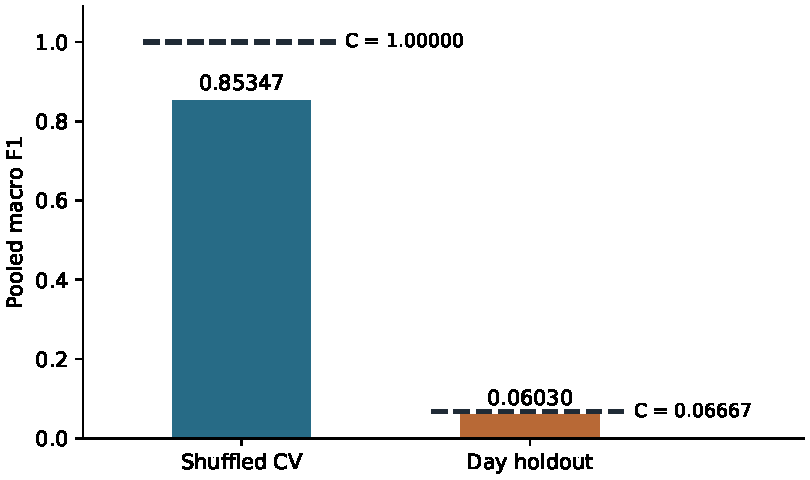
\includegraphics[width=0.95\columnwidth]{figures/cic_hero.pdf}
\caption{CICIDS2017 unweighted forest. Shuffled cross-validation has full label coverage; day holdout makes all fine-grained attack labels unavailable. The ceiling is a property of each protocol.}
\end{figure}

The day-held-out unweighted forest has benign recall 0.99858. Of the 557,646 unavailable attack rows, 475,727 are sent to benign and the remainder to other attack labels. Those other attack labels have zero covered support in the pooled score, so they provide free oracle destinations. This explains why the exact oracle equals the coverage ceiling here. The micro ceiling is 0.80300 because benign dominates the cohort. Merging web labels gives a 13-label ceiling of 0.07692; the declared eight-family mapping gives 0.25; binary attack detection has ceiling one. These are different evaluation targets.

\subsection{Fixed-cohort withholding and rankings}
The official UNSW-NB15 split has complete coverage. The unweighted forest's five-seed mean is 0.47144, with seed SD 0.00094. Training-label availability cannot explain that shortfall. Withholding two labels creates \(C=0.8\), but its oracle depends on their support and legal destinations. For Analysis plus Backdoor at seed 42, \(O=0.79833\) and \(F=0.47067\).

The covered-row calculations use a different label inventory for each withheld pair, while full scoring retains all test labels. The resulting rank-disagreement counts are descriptive properties of these two score definitions on this finite grid; they do not establish that either ranking is wrong. All 180 full scores match the earlier grid to absolute tolerance $10^{-12}$, and the new confusion matrices permit reconstruction of covered-row scores.

The post-hoc routing control is moved to the supplement. It uses the true availability status and illustrates how a prediction to an unscored label can affect support-scored F1; it is not evidence of improved recognition or a deployable unknown-attack rule.

\subsection{Natural fractional coverage and model families}
In adjacent-batch gas sensing, toluene is unavailable when batch 6 is tested. The batch-6 test fold contains 467 toluene rows; 1,759 is the pooled toluene support across all test batches. Thus 1,292 of 1,759 toluene test rows are in folds where toluene is available, giving \(\rho=1292/1759\). The other five classes have full coverage. Global label presence misses this fold-level restriction: all six labels occur somewhere in training.

\begin{table}[h]\centering
\caption{Different natural protocols retain their own targets. \(O-F\) is a score shortfall, not an estimate of model quality.}
\begin{tabular}{lrrr}
Case & C & O & F\\
NSL original, forest (seed 42) & 0.55263 & 0.55263 & 0.25456\\
CIC day, forest & 0.06667 & 0.06667 & 0.06030\\
Gas, forest & 0.97449 & 0.96222 & 0.57034\\
Gas, logistic & 0.97449 & 0.96222 & 0.61946\\
\end{tabular}\end{table}
The gas oracle is 0.01227 below the coverage ceiling. This difference is 3.0\% of the forest's gap \(C-F\) to the ceiling and 3.5\% of logistic regression's gap; the denominator is the model's shortfall from \(C\), not from one. It explains zero toluene hits in batch 6 but little of the pooled shortfall. Across all 19 gas fits, full and covered-only rankings agree exactly: Spearman and Kendall correlations are one, with 161 concordant comparisons and ten ties. The model-family contrast therefore provides no natural family-ranking reversal. CORAL logistic scores 0.63760 while retaining the same legal ceiling.

\subsection{Algorithm checks and literature screening}
Exhaustive row-level enumeration on 80 small seeded inputs agrees with both solvers under support and union scoring. Another 100 cases with explicitly supplied legal heads, including labels absent from training, agree with exhaustive predictions. A repeated-vocabulary check reduces 300 unavailable folds from \(2^{100}\) candidate assignments to two. These checks validate implementation and edge cases; fitted scores lying below a theorem are not independent evidence of significance. Varied synthetic shapes still reach exact-search budgets, as documented in the supplement.

A local protocol was committed before collecting six Crossref searches, each retaining the first 100 relevance-ranked records dated 2017--2026. Title filtering and DOI deduplication yielded 385 candidates. NumPy seed 20261108 selected 50 without replacement. The public frame, source metadata, sample, checksum and coding sheet are retained. This is a prospective local freeze rather than external preregistration.

Screening confirmed three eligible evaluations, excluded fourteen records and left thirty-three eligibility decisions unresolved. Temporal neuron coding and split learning were frequent reasons not to infer evaluation timing from a title. Of the three confirmed cases, one binary source-to-target evaluation permits both labels and therefore has legal ceiling one; its exact F1 averaging remains unresolved. The other two lack verified vocabulary/support/scoring information. No complete incompatible-score comparison is established. The result is a candidate-screening pilot, not a survey of fifty confirmed temporal IDS papers or a field prevalence estimate. Accessible abstract evidence can establish eligibility without establishing a score convention; missing evidence is retained as missing. The separate targeted source checks and DOI verification are in the supplement and artifact.

\section{Using the Diagnostic}
Choose the evaluation target before optimizing a split. Stratified shuffled cross-validation can measure interpolation over a shared inventory but does not establish future-day generalization. A chronological or capture-group holdout addresses a different deployment question and should retain the availability audit. Leave-one-attack-class-out should specify a binary alarm or a scored unknown target when the aim is unfamiliar-attack detection. Exact identification of a withheld fine-grained label cannot measure that capability for a training-restricted output head.

The reporting sequence is short: preserve fold membership; state the legal vocabulary and per-class support; declare pooling and the scored labels; compute \(C\), then \(O\) or its sandwich if destination loss matters; report full and covered-row scores with their respective inventories. State whether labels come from training or a global head. A ratio \(F/O\), when \(O>0\), describes attainment on that cohort only and should accompany the absolute score. It cannot make different targets or populations comparable.

The package exposes fold-array and count-based interfaces, accepts an explicit legal vocabulary per fold, and supplies a CLI for count files. Reproduction commands and a table-to-file map accompany the release. Counts, software, manifests and checksums are public artifacts; raw traffic redistribution remains subject to dataset terms.

\section{Limitations and Conclusion}
The simple ceiling is a scoring corollary of legal-output constraints. It does not measure feature separability, rare-class learnability, calibration or deployment utility. The exact oracle adds unavoidable false-positive loss and admits a vocabulary-parameterized algorithm, but this correction is small in the natural examples considered. The five-seed NSL-KDD comparison does not show a full-versus-covered mean winner change: kNN leads both under the examined pipelines. Its scores remain a fixed-split illustration, not a reanalysis of a published model comparison. Shared-cohort repetitions describe fixed experiments rather than population uncertainty.

The literature screening has a bounded search frame and unresolved sources. It cannot support a field-wide prevalence claim. No verified incompatible published score is established. Timestamped CIC files and corrected label releases are absent locally, and a file-verified CICDDoS2019 study is not supplied. A permanent DOI, an externally hosted anonymous artifact and independent reproduction also remain pending.

The main practical conclusion is narrower than a new detector claim: a benchmark score should be interpreted against the decisions its protocol permits. NSL-KDD shows natural partial coverage; CICIDS2017 shows an extreme day-holdout restriction; the gas comparison shows that coverage can explain little. Reporting these outcomes, including the null ranking result, makes the diagnostic useful without overstating its reach.

\section*{Data availability}
Dataset sources are cited above. The accompanying code release contains aggregate results, split manifests, hashes, source coding and commands mapped to the manuscript. Original data terms continue to apply.
\section*{Declarations}
This research received no funding. The author declares no financial or non-financial competing interests.
\section*{Use of generative AI}
Generative AI assisted code development, mathematical exposition, literature screening, analysis planning and manuscript editing. Numerical results were computed with the released scripts. The author retains responsibility for the submitted work.
\bibliographystyle{IEEEtran}
\bibliography{references}
\end{document}
